\section{Installation}
\label{tutorial_02}

\tick{\textbf{Goals:} The objective of this section is to guide you through downloading, installing and starting Rodin. In addition, we explain the update mechanisms needed to install new plugins for Rodin. Finally, we name the Rodin-specific GUI elements and describe their functions.
}

\tick{\textbf{You can skip this section, if\ldots}
\begin{itemize}
	\item \ldots you know how to install and update Rodin
	\item \ldots you know how to install new plugins for Rodin
\end{itemize}
}

\warning{Before installing Rodin, you should ensure that your computer fulfills the system requirements. The system requirements for the present release can be found in the Rodin Wiki (\ref{rodin_wiki}).}

\subsection{Install Rodin for the first time}

\subsubsection{Step 1: Download}

The first step is to download Rodin. Rodin is available for download at the Rodin Download page (\ref{rodin_download})

Rodin is available for Windows, Mac OS, and Linux.  No matter which platform you use, the distribution is always packed in a zip-file (\ref{zip_file}).  Download the zip file for your system anywhere on your PC.

\info{It is recommended that you download the latest stable version.}

\subsubsection{Step 2: Install and Run Rodin}

To install Rodin, extract the contents of the zip file in a desired folder. You can run the tool by using the \texttt{rodin} executable.

Starting Rodin should bring up the window as shown in figure \ref{fig_tut_02_workspace_launcher}. Here you can specify the path where Rodin stores your projects.

\begin{figure}[!h]
\begin{center}
	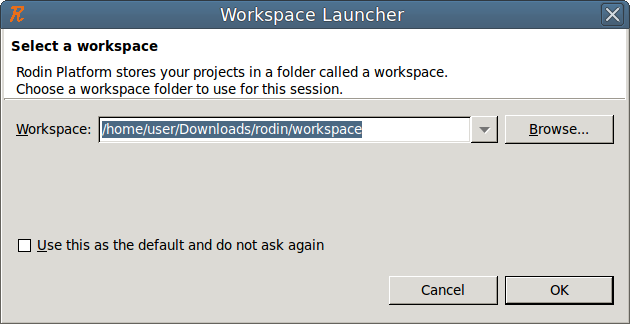
\includegraphics{img/tutorial/tut_02_install1.png}
	\caption{Eclipse Workspace Launcher}
	\label{fig_tut_02_workspace_launcher}
\end{center}
\end{figure}

After specifying a path click on the \textsf{OK} button. Rodin should start and bring up the window shown in figure \ref{fig_tut_02_rodin_gui}.

\warning{When using a Linux distribution, a Welcome window may open up. Exit out of this window to get to the main screen.}

\begin{figure}[!h]
\begin{center}
	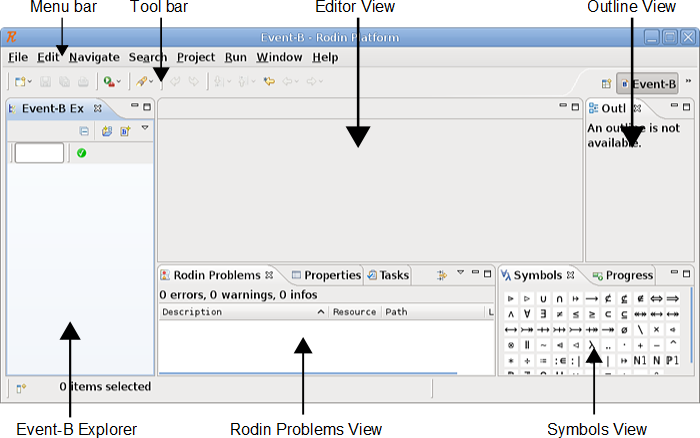
\includegraphics{img/tutorial/tut_02_install2.png}
	\caption{Rodin GUI}
	\label{fig_tut_02_rodin_gui}
\end{center}
\end{figure}

As already mentioned in Section \ref{subsection_eclipse}, the GUI of an Eclipse application consists of Views, Editors, Toolbars, Quickview, Perspectives and many more elements. We name the different Rodin GUI elements (i.e. Views) which are visible after starting Rodin for the first time and explain their functions:

\begin{description}
	\item[Menu bar (\ref{menu_bar})] The menu bar of Rodin provides for instance file and edit operations.
	\item[Tool bar (\ref{tool_bar})] The tool bar provides short cuts for familiar commands like save, print, undo and redo.
	\item[Event-B Explorer (\ref{eventb_explorer})] The Event-B Explorer shows the projects' (\ref{project}) tree structures. It has projects as main entries and for each one its corresponding project files.
	\item[Outline View (\ref{outline_view})] A view used to view the outline of the active editor or file respectively.
	\item[Rodin Problems view (\ref{rodin_problems_view})] The Rodin Problems View shows problems (i.e. syntax errors) in the active editor.
	\item[Symbols View (\ref{symbols_view})] A view that shows a list of available mathematical symbols which can be used in conjunction with the mathematical notation (\ref{mathematical_notation}).
	\item[Editor View (\ref{editor_view})] The editor view contains the active editor.
\end{description}

\subsection{Install new plugins}

This sections shows how to install new plugins for Rodin by using the example of the Atelier B Provers plugin (\ref{atelier_b_provers}). It is highly recommended to install this plugin because without it we will not be able to prove anything.

Open the Install Manager \textsf{Help $\rangle$ Install New Software\ldots}. Click the downward arrow next to the field \textsf{Work with} to select the Atelier~B Provers update site. Mark the Atelier~B Provers entry and click on the \textsf{Next} button (compare with figure \ref{fig_tut_02_install_manager}). Follow the installation instruction to install the plugin. After installing the plugin, you will be asked to restart Rodin in order to finalize the installation.

\begin{figure}[!h]
\begin{center}
	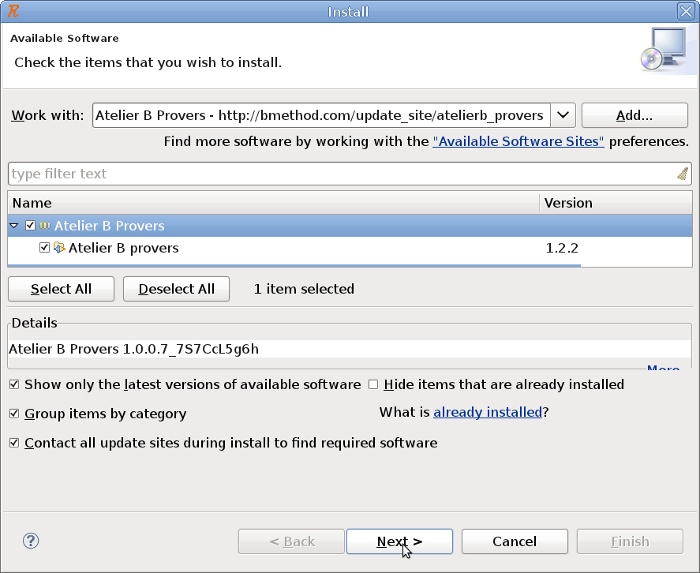
\includegraphics{img/tutorial/tut_02_install3.png}
	\caption{Eclipse Install Manager}
	\label{fig_tut_02_install_manager}
\end{center}
\end{figure}

